\section{First Order}
\label{chapter4}

We move on from the \emph{Propositional} level to the \emph{Predicate} or \emph{First Order} level of logic following \cite{goldblatt}'s \emph{first-principles} approach before changing course to \cite{lambekscott}'s \emph{BKJ Semantics} in order to better realize quantifiers in our topos of study.\newline
For our purposes we have chosen at this stage not to add multiple constants or predicates and to omit function symbols\footnote{any function symbol could be substituted with a relation or predicate symbol which specifies the function's \emph{graph}.}. Also we start off with a single \emph{sort} or \emph{type} of variables.\newline
\newline
We have also decided, for the purpose of this work, not to mention Soundness \& Completeness Theorems which generalize to first order level soundness \& completeness of topoi (\ref{soundcompl}) with respect to intuitionistic logic.\newline We leave as references chapter XI of \cite{goldblatt} and part II of \cite{lambekscott}. 


\newpage
\subsection{First Order Logic and Topoi}

In order to interpret an elementary language $\mathcal{L}$ in a topos $\mathcal{E}$ it is necessary first to reformulate Tarski Semantics for $\mathcal{L}$-terms and $\mathcal{L}$-formulae (which from now on will be called just 'terms' and 'formulae') in a given \emph{context}.
\begin{definition}[\emph{context}]
	We specify a \emph{context} for a formula $\phi$ by fixing an integer $m \geq 1$ which will be called \emph{appropriate} to $\phi$ if all the variables that occur in $\phi$ free or bound are all elements of the list $\{x_1,..,x_m\}$. We will refer to this $\phi$ as a \emph{formula-in-context}. \newline
	Similarly a \emph{term-in-context}  is a term \textbf{t} in which all occurrences of variables in \textbf{t} belong to $\{x_1,..,x_m\}$. 
\end{definition}

We re-define satisfaction for $\phi$ by $m$-length sequences $\{ \textbf{a}_1,..,\textbf{a}_m \}$ by requiring that $\mathcal{M} \vDash \phi[\textbf{a}_1,..,\textbf{a}_n]$ iff $\mathcal{M} \vDash \phi[\textbf{y}]$ for some assignment \textbf{y} for which $\textbf{y}_i = \textbf{a}_i$ whenever $x_i$ is free in $\phi$.  \newline
Note that given an $\mathcal{L}$-model $\mathcal{M}= \langle \textbf{A}, \textfrak{P}, \textfrak{c} \rangle$ and a \emph{context} $m \geq 1$, each formula-in-context $\phi$ determines a sub-set $\phi^m \subseteq \textbf{A}^m$ namely the set of all m-tuples satisfying $\phi$:
\begin{equation*}
	\phi^m = \{(a_1,..,a_m) : \mathcal{M} \vDash \phi[a_1,..,a_m]\}.
\end{equation*}
Note also that by this definition:
\begin{align*} 
	(\neg \phi)^m &=  \textbf{A} \setminus \phi^m \\ 
	(\phi \land \psi)^m &=  \phi^m \cap \psi^m. \\
	(\phi \lor \psi)^m &=  \phi^m \cup \psi^m. \\
	(\phi \Rightarrow \psi)^m &=  (\textbf{A} \setminus \phi^m) \cup \psi^m. \\ etc..
\end{align*}
This is a translation of $\mathcal{L}$-formulae into sub-sets or sub-objects of the product domain $\textbf{A}^m$ which in turn can be replaced by their characteristic functions $\llbracket \phi^m \rrbracket : \textbf{A}^m \rightarrow \textbf{2}$. \newline
With this in mind, we can finally generalize from $\mathbb{Set}$ to a generic topos.
\newline
\newline
Let $\mathcal{E}$ be a topos and a fixed $\mathcal{E}$-object  $\textfrak{a}$ \footnote{the fixed object corresponds to a fixed type or sort.}.\newline

We first give some preliminary definitions:
\begin{definition}[$\Delta_\textfrak{a}$ and $\delta_\textfrak{a}$ ]
	$\Delta_\textfrak{a} : \textfrak{a} \rightarrowtail \textfrak{a} \times \textfrak{a}$ is the product arrow $id_\textfrak{a} \times id_\textfrak{a}$.\newline
	$\delta_\textfrak{a} : \textfrak{a} \times \textfrak{a} \rightarrow \Omega$ is the characteristic arrow of $\Delta_\textfrak{a}$. 
\end{definition}

\begin{definition}[$true_\textfrak{o}$]
	For any $\mathcal{E}$-object \textfrak{o}, \newline
	$true_\textfrak{o}$ is the composite arrow $true \;\circ\; !_\textfrak{o}$ \newline
	(where $!_\textfrak{o}$ as usual is the unique arrow from \textfrak{o} to the terminal \textbf{1}).
	
\end{definition}


We are finally ready to define a topos-model or $\mathcal{E}$-model for First Order Logic:
(From now on we fix an appropriate $m \geq 1$ context).

\begin{definition}[$\mathcal{E}$-model] \footnote{note that we can generalize this definition by taking multiple objects in I (multiple sorts), multiple predicates in II and generalized elements in III.}
	An $\mathcal{E}$-model for $\mathcal{L}$ is a structure \textfrak{M}=$\langle \textfrak{a}, \textfrak{p}, \textfrak{f}_c \rangle$ where
	\begin{enumerate}[label=\Roman*]
		\item 	\;\;\textfrak{a} is an $\mathcal{E}$-object for the \emph{domain} that is \emph{not empty} i.e., $\mathcal{E}(\textbf{1},\textfrak{a})\neq \emptyset$.
		\item 	 \;\;\textfrak{p} 	:	$\textfrak{a}^n \rightarrow \Omega$ is an $\mathcal{E}$-arrow for the \emph{predicate/relation}. \footnote{we will assume $0 \leq n \leq m$.}
		\item 	\;\;$\textfrak{f}_c$	:	$\textbf{1} \rightarrow \textfrak{a}$ is an $\mathcal{E}$-\emph{element} of \textfrak{a} for the \emph{particular individual}.
	\end{enumerate}
\end{definition}

\begin{remark}
	Notice that if the arity of the predicate-arrow is $n=0$ we recover \emph{propositions}, if the arity is $n=1$ we obtain unary \emph{predicates} and if $n>1$ n-ary \emph{relations}. 
\end{remark}
We \emph{realize} i.e., interpret the terms \textbf{t} as arrows $\textfrak{a}^m \rightarrow \textfrak{a}$ :

\begin{definition}[$\llbracket \textbf{t} \rrbracket^m$]
	\begin{equation*}
		\llbracket \textbf{t} \rrbracket^m =
		\begin{cases}
			pr_i^m : \textfrak{a}^m \rightarrow \textfrak{a} & \text{if \textbf{t} is the variable $x_i$}\\
			\textfrak{f}_c \;\circ\; !_\textfrak{a} : \textfrak{a}^m \rightarrow \textfrak{a}  & \text{if \textbf{t} is the constant \textbf{c}}
		\end{cases}   
	\end{equation*}  
	For $m>1$ the $m$ variables in context $\{x_i\}_{i=1}^m$ are realized by the $m$ projections $pr_i^m$ from $\textfrak{a}^m$ to \textfrak{a}. \newline
	If $m=1$ the only variable in context $x = x_1$ is realized by the identity arrow $id_\textfrak{a}$.
\end{definition}


We now define for each $\mathcal{L}$-formula $\phi$ a realization/interpretation $\llbracket  \phi \rrbracket^m$ as an arrow $\textfrak{a}^m \rightarrow \Omega$:
\newline
(From now on $\llbracket  \phi \rrbracket, \llbracket  \textbf{t} \rrbracket $  will be used instead of $\llbracket  \phi \rrbracket^m, \llbracket  \textbf{t} \rrbracket^m$ if the context is already specified and there is no ambiguity).

\begin{definition}[$\llbracket  \phi \rrbracket$]
	The atomic formulae admit the following \emph{realizations}:
	\begin{enumerate}
		\item $\llbracket \textbf{t} \approx \textbf{u}  \rrbracket = \delta_\textfrak{a} \circ (\llbracket \textbf{t} \rrbracket \times \llbracket \textbf{u} \rrbracket$)  .
		\begin{figure}[h]
			\centering
			\begin{tikzcd}
				{\textfrak{a}^m} && {\textfrak{a}^2} \\
				\\
				&& \Omega
				\arrow["{\llbracket \textbf{t} \rrbracket \times \llbracket \textbf{u} \rrbracket}"', from=1-1, to=1-3]
				\arrow["{\delta_\textfrak{a}}"', from=1-3, to=3-3]
				\arrow["{\llbracket \textbf{t} \approx \textbf{u} \rrbracket}"', from=1-1, to=3-3]
			\end{tikzcd}\
		\end{figure}
		
		\item $\llbracket \textbf{P}(\textbf{t}_1,..,\textbf{t}_n) \rrbracket = \textfrak{p} \circ (\llbracket \textbf{t}_1 \rrbracket \times ...\times\llbracket \textbf{t}_n \rrbracket)$.
		\begin{figure}[h]
			\centering
			\begin{tikzcd}
				{a^m} && {a^n} \\
				\\
				&& \Omega
				\arrow["{\llbracket \textbf{t}_1 \rrbracket \times ...\times\llbracket \textbf{t}_n \rrbracket}", from=1-1, to=1-3]
				\arrow["p"', from=1-3, to=3-3]
				\arrow["{\llbracket \textbf{P}(\textbf{t}_1,..,\textbf{t}_n) \rrbracket}"', from=1-1, to=3-3]
			\end{tikzcd}
		\end{figure}
		
	\end{enumerate}
	The rest follow by induction:
	\begin{enumerate}
		\setcounter{enumi}{2}
		\item $\llbracket \phi \land \psi \rrbracket = \llbracket \phi \rrbracket \land \llbracket \psi \rrbracket = \land \circ (\llbracket \phi \rrbracket \times \llbracket \psi \rrbracket) $.
		\begin{figure}[h]
			\centering
			\begin{tikzcd}
				{a^m} && {\Omega \times \Omega} \\
				\\
				&& \Omega
				\arrow["{\llbracket \phi \rrbracket \times \llbracket \psi \rrbracket}", from=1-1, to=1-3]
				\arrow["\land"', from=1-3, to=3-3]
				\arrow["{\llbracket \phi \land \psi \rrbracket}"', from=1-1, to=3-3]
			\end{tikzcd}\
		\end{figure}
		\item $\llbracket \phi \lor \psi \rrbracket = \llbracket \phi \rrbracket \lor \llbracket \psi \rrbracket = \lor \circ (\llbracket \phi \rrbracket \times \llbracket \psi \rrbracket) $.
		
		\item $\llbracket \neg \phi \rrbracket = \neg \circ \llbracket \phi \rrbracket$.
		
		\item $\llbracket \phi \Rightarrow \psi \rrbracket = \llbracket \phi \rrbracket \Rightarrow \llbracket \psi \rrbracket =\; \Rightarrow \circ (\llbracket \phi \rrbracket \times \llbracket \psi \rrbracket) $.
	\end{enumerate}		

\end{definition}

We can now define $\mathcal{E}$-validity for a formula $\phi$ starting by what it means for \textfrak{M} to \emph{model} $\phi$ denoted by $\textfrak{M} \vDash_\mathcal{E} \phi$. \newline
Let $\phi = \phi(x_{i_1},..x_{i_n})$ be a formula-in-context and take any arrow $g: \textfrak{a}^n \rightarrow \textfrak{a}$ 	,we construct a product arrow $f: p_1 \times .. \times p_m$ where: ($pr_k^n$ as usual denotes the k-th projection from $\textfrak{a}^n$)
\begin{equation*}
	p_i =
	\begin{cases}
		pr_k^n : \textfrak{a}^n \rightarrow \textfrak{a} & \text{if } j=i_k \text{ for some } \  1 \leq k \leq n.\\
		g  & \text{otherwise}.
	\end{cases}   
\end{equation*}  
\textfrak{M} is thus an "$\mathcal{E}$-model of $\phi = \phi(x_{i_1},..x_{i_n})$" i.e., $\textfrak{M} \vDash_\mathcal{E} \phi$ if:

\begin{definition}[\textfrak{M} models $\phi(x_{i_1},..x_{i_n})$]
	\begin{equation*}
		\textfrak{M} \vDash_\mathcal{E} \phi\text{ iff }\llbracket \phi \rrbracket_\textfrak{M} = true_{\textfrak{a}^n}.
	\end{equation*}
		Where the arrow $\llbracket \phi \rrbracket_\textfrak{M} = true_{\textfrak{a}^n} : \textfrak{a}^n \rightarrow \Omega$ is defined as $ true_{\textfrak{a}^m} \circ f$:
	\begin{figure}[h]
		\centering
		\begin{tikzcd}
			{\textfrak{a}^n} && {\textfrak{a}^m} \\
			\\
			&& \Omega
			\arrow["f", from=1-1, to=1-3]
			\arrow["{\llbracket \phi \rrbracket}", from=1-3, to=3-3]
			\arrow["{\llbracket \phi \rrbracket_\textfrak{M}}"', from=1-1, to=3-3]
		\end{tikzcd}\
	\end{figure}
\end{definition}

By the categorical properties of the arrows $true_\textfrak{o}$ \footnote{by using the fact that any arrow "that factors through \emph{true} is \emph{true}".} we find that:

\begin{remark}
	$\llbracket \phi \rrbracket_\textfrak{M} = true_{\textfrak{a}^n}$ iff $\llbracket \phi \rrbracket = true_{\textfrak{a}^m}$ .
\end{remark}
Thus:
\begin{definition}[$\mathcal{E}$-validity] Let $\phi = \phi(x_{i_1},..x_{i_n})$ be a formula-in-context,	then: 
	\begin{equation*}
		\textfrak{M} \vDash_\mathcal{E} \phi \;\text{	iff	}\; \llbracket \phi \rrbracket = true_{\textfrak{a}^m} .
	\end{equation*}
	The formula $\phi$ is $\mathcal{E}$-valid i.e., $ \vDash_\mathcal{E} \phi $ if for every $\mathcal{E}$-model \textfrak{M} one has $ \textfrak{M}\vDash_\mathcal{E} \phi $.
\end{definition}



\subsection{\hl{Another look at $\mathcal{G}_3$ through Predicates}}
\label{anotherlook}

We continue making some considerations on our topos of \emph{bushes}/$\mathbb{FF}_2$ like the following:
\newline
Recall our discourse about external and internal topos-logic in the propositional case, we left off with the result about \emph{bushes}/$\mathbb{FF}_2$ being bivalent and non-Boolean.
\newline
The culprit was the definition of propositional semantics for topoi.
\newline
The propositional truth-values are given by the two arrows $\top$ and $\bot$ of $\mathbb{FF_2}(\textbf{1},\Omega)$ that pick out the two roots 't' and 'f' of $\Omega= \textbf{1} + \textbf{1}_\bot$: 

\begin{figure}[h]
	\centering
	\begin{subfigure}[h]{0.2\textwidth}
		\begin{tikzcd}
			{\textcolor{OliveGreen}{\bigcdot}} && 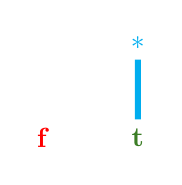
\begin{tikzpicture}[scale=0.4]
				\node (A) at (0,0) {\textcolor{red}{\textbf{f}}};
				\node (B) at (3,0) {\textcolor{OliveGreen}{\textbf{t}}};
				\node (C) at (3,3) {\textcolor{cyan}{$*$}};
				\draw[cyan, line width=.03in] (B) -- (C);
			\end{tikzpicture}
			\arrow["true", from=1-1, to=1-3]
		\end{tikzcd}
		\caption{$\top : \mathbf{1} \rightarrow \Omega$.}
	\end{subfigure}
	\hfil
	\centering
	\begin{subfigure}[h]{0.2\textwidth}
		\begin{tikzcd}
			{\textcolor{red}{\bigcdot}} && 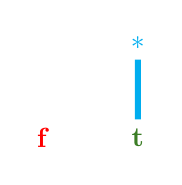
\begin{tikzpicture}[scale=0.4]
				\node (A) at (0,0) {\textcolor{red}{\textbf{f}}};
				\node (B) at (3,0) {\textcolor{OliveGreen}{\textbf{t}}};
				\node (C) at (3,3) {\textcolor{cyan}{$*$}};
				\draw[cyan, line width=.03in] (B) -- (C);
			\end{tikzpicture}
			\arrow["false", from=1-1, to=1-3]
		\end{tikzcd}
		\caption{$\bot : \mathbf{1} \rightarrow \Omega$.}
	\end{subfigure}
\end{figure} 


However, as in the case of $\mathbb{Set}$, truth values are meant to be \emph{generalized elements} of the sub-object classifier $\Omega$. The arrows from \textbf{1} to $\Omega$ are clearly insufficient to obtain the top element $*$ of $\textbf{1}_\bot \subset \Omega$. This is remedied if we take arrows from $\textbf{1}_\bot$. 
The object $\textbf{1}_\bot$ in fact is shown to be a \emph{representing object} for the category of \emph{bushes}.
\newline \newline
The hom-set $\mathbb{FF_2}(\textbf{1}_\bot,\Omega)$ has exactly three arrows which we denote by $\textfrak{p}_t, \textfrak{p}_f, \textfrak{p}_*$ each determined by the image of the top element of $\textbf{1}_\bot$.     


\begin{figure}[h]
	\centering
	\begin{tikzcd}
		
\begin{tikzpicture}[scale=0.4]
			\node (A) at (0,0) {\textcolor{OliveGreen}{$\bullet$}};
			\node (B) at (0,3) {\textcolor{OliveGreen}{$\bullet$}};
			\draw[OliveGreen, line width=.03in] (A) -- (B);
		\end{tikzpicture} && 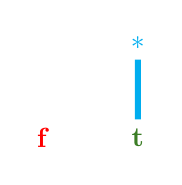
\begin{tikzpicture}[scale=0.4]
			\node (A) at (0,0) {\textcolor{red}{\textbf{f}}};
			\node (B) at (3,0) {\textcolor{OliveGreen}{\textbf{t}}};
			\node (C) at (3,3) {\textcolor{cyan}{$*$}};
			\draw[cyan, line width=.03in] (B) -- (C);
		\end{tikzpicture}
		\arrow["\textfrak{p}_t", from=1-1, to=1-3]
	\end{tikzcd}
	\caption{$\textfrak{p}_t : \mathbf{1}_\bot \rightarrow \Omega$. }
\end{figure}	

\begin{figure}[h]
	\centering
	\begin{tikzcd}
		
\begin{tikzpicture}[scale=0.4]
			\node (A) at (0,0) {\textcolor{red}{$\bullet$}};
			\node (B) at (0,3) {\textcolor{red}{$\bullet$}};
			\draw[red, line width=.03in] (A) -- (B);
		\end{tikzpicture} && 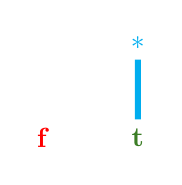
\begin{tikzpicture}[scale=0.4]
			\node (A) at (0,0) {\textcolor{red}{\textbf{f}}};
			\node (B) at (3,0) {\textcolor{OliveGreen}{\textbf{t}}};
			\node (C) at (3,3) {\textcolor{cyan}{$*$}};
			\draw[cyan, line width=.03in] (B) -- (C);
		\end{tikzpicture}
		\arrow["\textfrak{p}_f", from=1-1, to=1-3]
	\end{tikzcd}
	\caption{$\textfrak{p}_f : \mathbf{1}_\bot \rightarrow \Omega$. }
\end{figure}	


\begin{figure}[h]
	\centering
	\begin{tikzcd}
		
\begin{tikzpicture}[scale=0.4]
			\node (A) at (0,0) {\textcolor{OliveGreen}{$\bullet$}};
			\node (B) at (0,3) {\textcolor{cyan}{$\bullet$}};
			\draw[cyan, line width=.03in] (A) -- (B);
		\end{tikzpicture} && 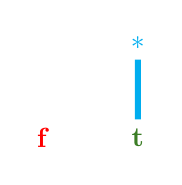
\begin{tikzpicture}[scale=0.4]
			\node (A) at (0,0) {\textcolor{red}{\textbf{f}}};
			\node (B) at (3,0) {\textcolor{OliveGreen}{\textbf{t}}};
			\node (C) at (3,3) {\textcolor{cyan}{$*$}};
			\draw[cyan, line width=.03in] (B) -- (C);
		\end{tikzpicture}
		\arrow["\textfrak{p}_*", from=1-1, to=1-3]
	\end{tikzcd}
	\caption{$\textfrak{p}_* : \mathbf{1}_\bot \rightarrow \Omega$. }
\end{figure}	

Note that these arrows can be viewed as realizations of unary \emph{predicates} which we name: $\textbf{P}_t,\textbf{P}_f,\textbf{P}_*$. 
\newline
Consider the following $\mathcal{E}$-model \textfrak{X} with specified context $m = 1$:
\begin{ex} (m=1)
	\begin{gather*}
		\textfrak{X}= \langle \textbf{1}_\bot, \{\textfrak{p}_t, \textfrak{p}_f, \textfrak{p}_*\}, \textfrak{f}_c \rangle. \\ \\
		\llbracket x \rrbracket = id_{\textbf{1}_\bot}: \textbf{1}_\bot \rightarrow \textbf{1}_\bot. \\ \llbracket \textbf{c} \rrbracket = \textfrak{f}_c \circ !_{\textbf{1}_\bot} : \textbf{1}_\bot \rightarrow \textbf{1}_\bot \; \text{ i.e., the constant map on the root of $\textbf{1}_\bot$}.  \\
		\llbracket \textbf{P}_t (x) \rrbracket = \textfrak{P}_t \circ \llbracket x \rrbracket = \textfrak{P}_t : \textbf{1}_\bot \rightarrow \Omega.\\
		\llbracket \textbf{P}_f (x) \rrbracket = \textfrak{P}_f \circ \llbracket x \rrbracket = \textfrak{P}_f : \textbf{1}_\bot \rightarrow \Omega.\\
		\llbracket \textbf{P}_* (x) \rrbracket = \textfrak{P}_* \circ \llbracket x \rrbracket = \textfrak{P}_* : \textbf{1}_\bot \rightarrow \Omega. 
	\end{gather*}
\end{ex}
Note that by construction $\textfrak{P}_t = true_{\textbf{1}_\bot}$ and so we have $\textfrak{X} \vDash_\mathcal{E} \textbf{P}_t(x) $. 
\newline
If we now compose these predicates with truth-arrows, we obtain:
\begin{gather*}
	\llbracket \neg \textbf{P}_t (x) \rrbracket = \neg \circ \llbracket \textbf{P}_t (x) \rrbracket = \neg \circ  \textfrak{P}_t = \textfrak{P}_f = \llbracket \textbf{P}_f (x) \rrbracket.\\
	\llbracket \neg \textbf{P}_* (x) \rrbracket = \neg \circ \llbracket \textbf{P}_* (x) \rrbracket = \neg \circ  \textfrak{P}_* = \textfrak{P}_f = \llbracket \textbf{P}_f (x) \rrbracket.\\
	\llbracket \neg \textbf{P}_f (x) \rrbracket = \neg \circ \llbracket \textbf{P}_f (x) \rrbracket = \neg \circ  \textfrak{P}_f = \textfrak{P}_t = \llbracket \textbf{P}_t (x) \rrbracket.
\end{gather*}

\begin{figure}[h]
	\centering
	\begin{tikzcd}
		
\begin{tikzpicture}[scale=0.4]
			\node (A) at (0,0) {\textcolor{red}{$\bullet$}};
			\node (B) at (0,3) {\textcolor{red}{$\bullet$}};
			\draw[red, line width=.03in] (A) -- (B);
		\end{tikzpicture} && 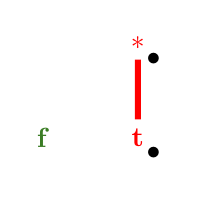
\begin{tikzpicture}[scale=0.4]
			\node (A) at (0,0) {\textcolor{OliveGreen}{\textbf{f}}};
			\node (B) at (3,0) {\textcolor{red}{\textbf{t}}};
			\node (b) at (3.5,-0.5) {\textcolor{black}{$\bullet$}};
			\node (C) at (3,3) {\textcolor{red}{$*$}};
			\node (c) at (3.5,2.5) {\textcolor{black}{$\bullet$}};
			\draw[red, line width=.03in] (B) -- (C);
		\end{tikzpicture}\\
		\\
		&& 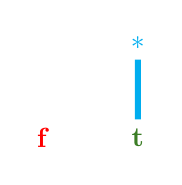
\begin{tikzpicture}[scale=0.4]
			\node (A) at (0,0) {\textcolor{red}{\textbf{f}}};
			\node (B) at (3,0) {\textcolor{OliveGreen}{\textbf{t}}};
			\node (C) at (3,3) {\textcolor{cyan}{$*$}};
			\draw[cyan, line width=.03in] (B) -- (C);
		\end{tikzpicture}
		\arrow["{\llbracket \textbf{P}_*(x)\rrbracket}", from=1-1, to=1-3]
		\arrow["\neg", from=1-3, to=3-3]
		\arrow["{\llbracket \neg\textbf{P}_*(x)\rrbracket}"', from=1-1, to=3-3]
	\end{tikzcd}
	\caption{$\llbracket \neg\textbf{P}_*(x)\rrbracket : \textbf{1}_\bot \rightarrow \Omega$.  The usual coloring notation is applied for this arrow. The images of the nodes of $\textbf{1}_\bot$ by $\llbracket \textbf{P}_*(x)\rrbracket$ are also shown as black bullets.}
\end{figure}	

\begin{gather*}
	\llbracket \textbf{P}_* (x) \land \textbf{P}_t (x) \rrbracket = \land \circ (\llbracket \textbf{P}_* (x) \rrbracket \times \llbracket \textbf{P}_t (x) \rrbracket) = \textfrak{P}_*. \\
	etc.. \\ \\
	\llbracket \textbf{P}_* (x) \lor \textbf{P}_t (x) \rrbracket = \lor \circ (\llbracket \textbf{P}_t (x) \rrbracket \times \llbracket \textbf{P}_* (x) \rrbracket) = \textfrak{P}_t. \\
	etc.. \\ \\
	\llbracket \textbf{P}_t (x) \Rightarrow \textbf{P}_* (x) \rrbracket = \Rightarrow \circ (\llbracket \textbf{P}_t (x) \rrbracket \times \llbracket \textbf{P}_* (x) \rrbracket) = \textfrak{P}_*. \\
	etc..
\end{gather*}
\newpage
\begin{remark}
	Again we find the (propositional) truth functions of $\mathcal{G}_3$.
	Though this time \emph{internally} by composition of the \emph{new} truth arrows for First Order Logic that we defined. In this case, these arrows are of the form $\textbf{1}_\bot \rightarrow \Omega$ which is precisely what we need for generalized elements of $\mathbb{FF_2}$. 
\end{remark}
 
Notice that $\textbf{P}_t$,$\textbf{P}_*$ and $\textbf{P}_f$ can also be viewed as characteristic arrows for the sub-forests $\{\textbf{1}_\bot\}$, $\{\bot\}$ and $\emptyset$ respectively.
\newline
This leads to the following consideration:
\begin{remark}
	What we found with these predicates is an application of the duality between \emph{bushes} $\mathbb{FF_2}$ and $(\mathbb{G_3})_{fin}$. \newline
	 $Sub(\textbf{1}_\bot)$ is isomorphic (as Gödel Algebras) to $C_3$ the 3-element chain which semantically characterizes our logic $\mathcal{G}_3$ i.e., $C_3 \models \mathcal{G}_3$.
\end{remark}


\newpage

\section{\hl{What about Quantifiers?}}
\label{whataboutquant}
To treat First Order Logic and \emph{quantifiers} we leave aside the method in \cite{goldblatt} we introduced earlier and instead apply a new approach outlined in \cite{lambekscott}, inspired by \emph{type theory} and the \emph{Curry-Howard} correspondence between objects and types, and arrive at a few conclusions.

\subsection{A Type-Theoretic Approach}

We introduce some new jargon:\newline
(The notation $\langle a,b \rangle$ is equivalent to $a \times b$.)	

\begin{itemize}
	\item The \emph{special} type $\Omega$ is the object $\Omega$.
	\item Variables of type $A_i$  i.e., $x_i:A_i$ are realized as \emph{indeterminate} arrows $1 \xrightarrow{x_i} A_i.$ 
	\item From  ($a:A$) $1 \xrightarrow{a} A$  and ($b:B$) $1 \xrightarrow{b} B$  one obtains  
	($\langle a,b \rangle : A \times B$)  $1 \xrightarrow{\langle a,b \rangle} A \times B$.
	\item $a=a'$ denotes \emph{internal} equality\footnote{as a first order relation.} and is realized as\footnote{recall that $\delta_A$  characteristic arrow of $\langle id_{A},id_{A} \rangle$.} 
	$1\xrightarrow{\langle a,a' \rangle}A \times A \xrightarrow{\delta_A}\Omega$.
	\item $\cdot = \cdot$ instead denotes \emph{external} equality\footnote{as equality of arrows.} between arrows in the topos.
	\item $\textfrak{T} \models p$ means that the topos \textfrak{T} satisfies the proposition $p$: In which case $p \cdot = \cdot \top$ as arrows in \textfrak{T}.	 
\end{itemize}
	
\begin{definition}[realization of $\phi(x)$]
	A predicate formula $\phi(x)$ which takes as argument an $x:A$ is realized as $1 \xrightarrow{x} A \xrightarrow{f} \Omega$ i.e., $\ulcorner \phi(x) \urcorner \equiv fx$ where $f = \ulcorner \phi \urcorner$ is the realization of the predicate $\phi$.
\end{definition}

Generalizing to an arbitrary context:

\begin{definition}[realization of $\psi(x_1,..,x_n)$]
	$\psi(x_1,x_2,...,x_n)$ with  $h = \ulcorner \psi \urcorner$ the realization of the n-ary predicate $\psi$ and $x_i : A_i$  is realized as \newline
	$1 \xrightarrow{\langle x_1,..,x_n \rangle} A_1 \times ... \times A_n \xrightarrow{h} \Omega$ .
\end{definition}

\begin{definition}[realization of $\phi(a)$]
	We extend this notion to $\ulcorner \phi(a) \urcorner \equiv f a$ realized as $C \xrightarrow{a} A \xrightarrow{f} \Omega$ (by a slight abuse of notation) where $a$ is one of the \emph{generalized elements} of $A$ at stage $C$.	
\end{definition}

Generalizing to an arbitrary context:

\begin{definition}[realization of $\psi(a_1,..,a_n)$]
	 $\psi(a_1,a_2,...,a_n)$ with generalized elements $C \xrightarrow{a_i} A_i$ at stage $C$ is realized as
	 $C \xrightarrow{\langle a_1,a_2..,a_n \rangle} A_1 \times ... \times A_n \xrightarrow{h} \Omega$.
\end{definition}


\begin{definition}[truth at a stage]
	$\phi(a)$ \emph{holds at stage C} or \emph{C forces $\phi(a)$} denoted by $C \VDashA \phi(a) $ if the following diagram commutes:
	\begin{figure}[h]
		\centering
		\begin{tikzcd}
			C & A & \Omega \\
			& 1
			\arrow["a", from=1-1, to=1-2]
			\arrow["f", from=1-2, to=1-3]
			\arrow["{!_C}"',dotted, from=1-1, to=2-2]
			\arrow["\top"', from=2-2, to=1-3]
		\end{tikzcd}\
		\caption{$f \; a \cdot = \cdot \top \; !_C $}	
	\end{figure}
	\newline
In general:
$\psi(a_1,..,a_n)$ \emph{holds at stage C} or \emph{C forces $\psi(a_1,..,a_n)$} denoted by $C \VDashA \psi(a_1,..,a_n) $ if the following diagram commutes:
\begin{figure}[h]
	\centering
	\begin{tikzcd}
		C && {A_1 \times .. \times A_n} && \Omega \\
		&& 1
		\arrow["h", from=1-3, to=1-5]
		\arrow["{\langle a_1,a_2,..,a_n\rangle}", dashed, from=1-1, to=1-3]
		\arrow["{!_C}"', dotted, from=1-1, to=2-3]
		\arrow["\top"', from=2-3, to=1-5]
	\end{tikzcd}
	\caption{$h \; \langle a_1,a_2,..,a_n\rangle \cdot = \cdot \top \; !_C $}	
\end{figure}
 
\end{definition}


As a consequence of these definitions the following hold:
\begin{prop}
	\begin{enumerate}
		\item If $C \VDashA \phi(a)$ and $D \xrightarrow{h} C$ then $D \VDashA \phi(ah)$. \footnote{by $ah$ we mean $a \circ h$ generalized element of $A$ at stage $D$.}
		\item If $h: D \twoheadrightarrow C $ is an epi and $D \VDashA \phi(ah)$, then $C \VDashA \phi(a)$. 
	\end{enumerate}
\end{prop}

We wish to characterize \emph{truth} in a topos as \emph{truth} at all stages and for all generalized elements.\newline

We can do better by restricting the stages:

\begin{definition}[generating set]
	A set $\mathcal{C}$ of objects of \textfrak{T} is a \emph{generating set} if for any two arrows $f,g :A \rightarrow B$ we have $f \cdot = \cdot g$ iff for all $C\in \mathcal{C}$ and all $C \xrightarrow{h} A$
	$fh \cdot = \cdot gh$.
\end{definition} 

\begin{definition}[truth in \textfrak{T}]
	A formula $\phi(x)$ is \emph{true} in a topos \textfrak{T} denoted by $\models_{\textfrak{T}} \phi(x)$ iff for all objects $C \in \mathcal{C}$ and all generalized elements $C \xrightarrow{a} A$ of $A$ at stage $C$, $C \VDashA \phi(a)$. 
\end{definition}

We also give a preliminary definition that will come in useful:

\begin{definition}[indecomposable]
	The object $C$ is \emph{indecomposable} if for all arrows $D \xrightarrow{k} C$ and $E \xrightarrow{l} C$ such that $[k,l]: D+E \twoheadrightarrow C$ \footnote{the notation $[k,l]$ is equivalent to $k+l$ the unique arrow from the co-product.} is an epi, either $k$ or $l$ is an epi.
\end{definition} 

The so-called \emph{Beth-Kripke-Joyal} Semantics, which we will use, are given by:

\begin{definition}[BKJ Semantics]
	Given $C \xrightarrow{a} A$ generalized element of the topos \textfrak{T}:
	\begin{enumerate}[label=(\roman*)]
		\item $C \VDashA a$ (in case $A=\Omega$) iff $a \cdot = \cdot \top !_C$. 
		\item $C \VDashA \top$ always holds. \footnote{this can be also thought as \emph{there is always an arrow-witness from C}.}
		\item $C \VDashA \bot$ iff $C \cong 0$ i.e., is an initial object in \textfrak{T}. \footnote{in our case of \emph{bushes} this would be the empty forest which can only give the \emph{trivial} generalized element.}
		\item $C \VDashA \phi(a) \land \psi(a)$ iff $C \VDashA \phi(a) $ and $C \VDashA \psi(a)$.
		\item $C \VDashA \phi(a) \lor \psi(a)$ iff there is an epi $[k,l]: D+E \twoheadrightarrow C$ such that $D \VDashA \phi(ak)$ and $E \VDashA \psi(al)$.
		\item $C \VDashA \phi(a) \Rightarrow \psi(a)$ iff for all $D \xrightarrow{h} C$ if $D \VDashA \phi(ah)$ then $D \VDashA \psi(ah)$.
		\item $C \VDashA \neg\phi(a)$ iff for all $D \xrightarrow{h} C$ if $D \VDashA \phi(ah)$ then $D \cong 0$.
	\end{enumerate}
	However, if $C$ is indecomposable, then we can replace (v) with the much simpler:
	\begin{enumerate}[label=(\roman*)']
		\setcounter{enumi}{4}
		\item $C \VDashA \phi(a) \lor \psi(a)$ iff either $C \VDashA \phi(a)$ or $C \VDashA \psi(a)$.
	\end{enumerate} 

\newpage	 
What interests us above all are the semantics for quantifiers where variables range over some sort.
We give the definitions for the cases of unary predicates and binary relations and leave implicit the successive generalizations for arbitrary arities.
	\newline
	 (In this case we quantify over $x:A$) :
\begin{enumerate}[label=(\roman*)]
	\setcounter{enumi}{6}
	\item $C \VDashA \forall_{x : A} \phi(x)$ iff, for all generalized elements $C \xrightarrow{a} A$, then $C \VDashA \phi(a)$.
	\item $C \VDashA \exists_{x : A} \phi(x)$ iff there is a generalized element $C \xrightarrow{a} A$ such that $C \VDashA \phi(a)$.
\end{enumerate}
	(If we introduce an additional variable or \emph{parameter} $y : B$  one has:)
	\begin{gather*}
		\ulcorner \phi(y,x) \urcorner \equiv g \langle y,x \rangle\\
		\ulcorner \phi(y,a) \urcorner \equiv g \; \langle y !_C, a \rangle \text{ with }\ulcorner \phi \urcorner \equiv g: B \times A \rightarrow \Omega
	\end{gather*}
	\begin{enumerate}[label=(\roman*)']
	 \setcounter{enumi}{6}
	\item $C \VDashA \forall_{y : B} \psi(y,a)$ iff, for all $D \xrightarrow{h} C$ and $D \xrightarrow{b} B$, then $D \VDashA \psi(b,ah)$.
	\item $C \VDashA \exists_{y : B} \psi(y,a)$ iff there is an epi $h : D\twoheadrightarrow C$ and a $D \xrightarrow{b} B$ such that $D \VDashA \psi(b,ah)$.
	\end{enumerate}
\end{definition}

\newpage
\subsection{\hl{Quantifying Predicates}}

Let's re-interpret the predicate symbols $p_t, p_*, p_f$ in this environment.
\newline
These are still arrows in $\mathbb{FF_2}$ of the form $\textfrak{p}_t, \textfrak{p}_*,\textfrak{p}_f  :\textbf{1}_\bot \rightarrow \Omega$.
\begin{remark}
	The predicates in question are $p_t(x), p_*(x), p_f(x)$ with $x : \textbf{1}_\bot$ variable of type $\textbf{1}_\bot$.
\end{remark}
Remembering from (\ref{representing}) that in our topos $\mathbb{FF_2}$ we have that $\textbf{1}_\bot$ is also the representing object i.e., $\mathbb{FF_2}(\textbf{1}_\bot, F) \cong |F|$, we can restrict ourselves to the only stage given by $\textbf{1}_\bot$ and let the \emph{generating set} be $\mathcal{C}:=\{\textbf{1}_\bot\}$.
\begin{ex}
What does it mean for say $p_*(x)$ to be \emph{true} at stage $\textbf{1}_\bot$ for some generalized element $\textbf{1}_\bot \xrightarrow{a_0} \textbf{1}_\bot$ i.e., $\textbf{1}_\bot \VDashA p_*(a_0)$? We require the following diagram to commute.

%\begin{tikzcd}
%		\begin{tikzpicture}[scale=0.4]
%		\node (a) at (0.5,-1) {\textcolor{Plum}{$\bullet$}};
%		\node (b) at (0.5,2) {\textcolor{Plum}{$\bullet$}};
%		\draw[Plum, line width=.03in] (a) -- (b);
%	\end{tikzpicture} && 	\begin{tikzpicture}[scale=0.4]
%	\node (a) at (0.5,-1) {\textcolor{Plum}{$\bullet$}};
%	\node (b) at (0.5,2) {\textcolor{Lavender}{$\bullet$}};
%	\draw[Lavender, line width=.03in] (a) -- (b);
%	\end{tikzpicture}
%	\arrow["{a_0}", from=1-1, to=1-3]
%\end{tikzcd}
%
%\begin{tikzcd}
%	\begin{tikzpicture}[scale=0.4]
%		\node (a) at (0.5,-1) {\textcolor{Plum}{$\bullet$}};
%		\node (b) at (0.5,2) {\textcolor{Lavender}{$\bullet$}};
%		\draw[Lavender, line width=.03in] (a) -- (b);
%	\end{tikzpicture} && 	\begin{tikzpicture}[scale=0.4]
%		\node (a) at (0.5,-1) {\textcolor{Plum}{$\bullet$}};
%		\node (b) at (0.5,2) {\textcolor{Lavender}{$\bullet$}};
%		\draw[Lavender, line width=.03in] (a) -- (b);
%	\end{tikzpicture}
%	\arrow["{a_1}", from=1-1, to=1-3]
%\end{tikzcd}


\begin{figure}[h]
	\centering
	\begin{tikzcd}
			
\begin{tikzpicture}[scale=0.4]
			\node (A) at (0,0) {\textcolor{OliveGreen}{$\bigcdot$}};
			\node (a) at (0.5,0) {\textcolor{Plum}{$\bullet$}};
			\node (B) at (0,3) {\textcolor{OliveGreen}{$\bigcdot$}};
			\node (b) at (0.5,3) {\textcolor{Lavender}{$\bullet$}};
			\draw[OliveGreen, line width=.03in] (A) -- (B);
		\end{tikzpicture} & 	
\begin{tikzpicture}[scale=0.4]
		\node (A) at (0,0) {\textcolor{OliveGreen}{$\bigcdot$}};
		\node (a) at (0.5,0) {\textcolor{Plum}{$\bullet$}};
		\node (b) at (0.5,0.5) {\textcolor{Lavender}{$\bullet$}};
		\node (B) at (0,3) {\textcolor{cyan}{$\bigcdot$}};
		\draw[cyan, line width=.03in] (A) -- (B);
		\end{tikzpicture} & 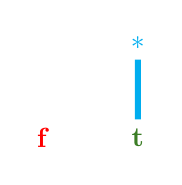
\begin{tikzpicture}[scale=0.4]
		\node (A) at (0,0) {\textcolor{red}{\textbf{f}}};
		\node (B) at (3,0) {\textcolor{OliveGreen}{\textbf{t}}};
		\node (C) at (3,3) {\textcolor{cyan}{$*$}};
		\draw[cyan, line width=.03in] (B) -- (C);
		\end{tikzpicture} \\
		& 	\begin{tikzpicture}[scale=0.4]
			\node (A) at (0,0) {\textcolor{OliveGreen}{$\bigcdot$}};
		\end{tikzpicture}
		\arrow["{a_0}", from=1-1, to=1-2]
		\arrow["\textfrak{p}_*", from=1-2, to=1-3]
		\arrow["{!_{\textbf{1}_\bot}}"', from=1-1, to=2-2]
		\arrow["\top"', from=2-2, to=1-3]
	\end{tikzcd}
	\caption{ $\textfrak{p}_* a_0 \cdot = \cdot \top !_{\textbf{1}_\bot} $ }
\end{figure}
Of course, taking the other generalized element  $\textbf{1}_\bot \xrightarrow{a_1} \textbf{1}_\bot$ the diagram fails to commute so $\textbf{1}_\bot \nVDash p_*(a_1)$.
\begin{figure}[h]
	\centering
	\begin{tikzcd}
		
\begin{tikzpicture}[scale=0.4]
			\node (A) at (0,0) {\textcolor{OliveGreen}{$\bigcdot$}};
			\node (a) at (0.5,0) {\textcolor{Plum}{$\bullet$}};
			\node (B) at (0,3) {\textcolor{OliveGreen}{$\bigcdot$}};
			\node (b) at (0.5,3) {\textcolor{Lavender}{$\bullet$}};
			\draw[OliveGreen, line width=.03in] (A) -- (B);
		\end{tikzpicture} & 	
\begin{tikzpicture}[scale=0.4]
			\node (A) at (0,0) {\textcolor{OliveGreen}{$\bigcdot$}};
			\node (a) at (0.5,0) {\textcolor{Plum}{$\bullet$}};
			\node (b) at (0.5,3) {\textcolor{Lavender}{$\bullet$}};
			\node (B) at (0,3) {\textcolor{cyan}{$\bigcdot$}};
			\draw[cyan, line width=.03in] (A) -- (B);
		\end{tikzpicture} & 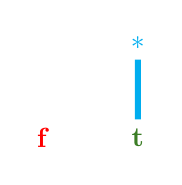
\begin{tikzpicture}[scale=0.4]
			\node (A) at (0,0) {\textcolor{red}{\textbf{f}}};
			\node (B) at (3,0) {\textcolor{OliveGreen}{\textbf{t}}};
			\node (C) at (3,3) {\textcolor{cyan}{$*$}};
			\draw[cyan, line width=.03in] (B) -- (C);
		\end{tikzpicture} \\
		& 	\begin{tikzpicture}[scale=0.4]
			\node (A) at (0,0) {\textcolor{OliveGreen}{$\bigcdot$}};
		\end{tikzpicture}
		\arrow["{a_1}", from=1-1, to=1-2]
		\arrow["\textfrak{p}_*", from=1-2, to=1-3]
		\arrow["{!_{\textbf{1}_\bot}}"', from=1-1, to=2-2]
		\arrow["\top"', from=2-2, to=1-3]
	\end{tikzcd}
	\caption{ $\textfrak{p}_* a_1 \cdot \neq \cdot \top !_{\textbf{1}_\bot} $ }
\end{figure}

By the previous considerations we conclude that:
\begin{gather*}
	\not\models_{\mathbb{FF_2}} p_*(x). \;\;\;\;
	\not\models_{\mathbb{FF_2}} p_f(x). \;\;\;\;
	\models_{\mathbb{FF_2}} p_t(x).
\end{gather*}

\end{ex}

What happens now if we quantify over $(x:\textbf{1}_\bot)$?

\begin{ex}
	For $\textbf{1}_\bot \VDashA \forall_{x:1_\bot} p_*(x)$ we need to check whether $\textbf{1}_\bot \VDashA p_*(a)$ for all $\textbf{1}_\bot \xrightarrow{a} \textbf{1}_\bot$.
	\begin{figure}[h]
		\centering
		\begin{tikzcd}
			
\begin{tikzpicture}[scale=0.4]
				\node (A) at (0,0) {\textcolor{black}{$\bigcdot$}};
				\node (B) at (0,3) {\textcolor{black}{$\bigcdot$}};
				\draw[black, line width=.03in] (A) -- (B);
			\end{tikzpicture} & 	
\begin{tikzpicture}[scale=0.4]
			\node (A) at (0,0) {\textcolor{OliveGreen}{$\bigcdot$}};
			\node (B) at (0,3) {\textcolor{cyan}{$\bigcdot$}};
			\draw[cyan, line width=.03in] (A) -- (B);
			\end{tikzpicture} &  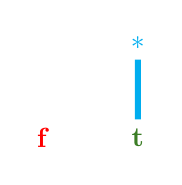
\begin{tikzpicture}[scale=0.4]
			\node (A) at (0,0) {\textcolor{red}{\textbf{f}}};
			\node (B) at (3,0) {\textcolor{OliveGreen}{\textbf{t}}};
			\node (C) at (3,3) {\textcolor{cyan}{$*$}};
			\draw[cyan, line width=.03in] (B) -- (C);
			\end{tikzpicture} \\
			& \begin{tikzpicture}[scale=0.4]
				\node (A) at (0,0) {\textcolor{OliveGreen}{$\bigcdot$}};
			\end{tikzpicture}
			\arrow["{a_0}", curve={height=6pt}, from=1-1, to=1-2]
			\arrow["\textfrak{p}_*", from=1-2, to=1-3]
			\arrow["{!_{\textbf{1}_\bot}}"', from=1-1, to=2-2]
			\arrow["\top"', from=2-2, to=1-3]
			\arrow["{a_1}", curve={height=-6pt}, from=1-1, to=1-2]
		\end{tikzcd}
	\end{figure}
	\newline
	We find, without surprises, that:
	\begin{gather*}
		\not\models_{\mathbb{FF_2}} \forall_{x:1_\bot} p_f(x). \;\;\;\;
		\not\models_{\mathbb{FF_2}} \forall_{x:1_\bot} p_*(x). \;\;\;\;
		\models_{\mathbb{FF_2}} \forall_{x:1_\bot} p_t(x).
	\end{gather*}

Moving on to existentials:
\newline	
	For $\textbf{1}_\bot \VDashA \exists_{x:1_\bot}\textfrak{p}_*(x)$ we need to check whether $\textbf{1}_\bot \VDashA p_*(a)$ for some $\textbf{1}_\bot \xrightarrow{a} \textbf{1}_\bot$.
	We find:
\begin{gather*}
		\not\models_{\mathbb{FF_2}} \exists_{x:1_\bot} p_f(x). \;\;\;\;
		\models_{\mathbb{FF_2}} \exists_{x:1_\bot} p_*(x). \;\;\;\;
		\models_{\mathbb{FF_2}} \exists_{x:1_\bot} p_t(x).
\end{gather*}
\end{ex}


\newpage
\subsection{\hl{Quantifying Relations}}
	 		 
In a new example, we introduce a \emph{relation} symbol $r$.
 \newline
This is realized as an arrow \textfrak{r} from $\textbf{1}_\bot \times \textbf{1}_\bot$ to $\Omega$ ($x$ and $y$ have both the same type $1_\bot$) of the following form:

\begin{figure}[h]
	\centering
	\begin{tikzcd}
		
\begin{tikzpicture}[scale=0.35]
			\node (A) at (0,0) {\textcolor{OliveGreen}{$\bigcdot$}};
			\node (B) at (-3,3) {\textcolor{OliveGreen}{$\bigcdot$}};
			\node (C) at (0,3) {\textcolor{OliveGreen}{$\bigcdot$}};
			\node (D) at (3,3) {\textcolor{cyan}{$\bigcdot$}};
			\draw[OliveGreen, line width=.03in] (A) -- (B);
			\draw[OliveGreen, line width=.03in] (A) -- (C);
			\draw[cyan, line width=.03in] (A) -- (D);
		\end{tikzpicture} && 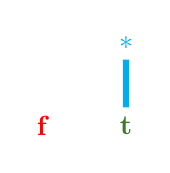
\begin{tikzpicture}[scale=0.35]
			\node (A) at (0,0) {\textcolor{red}{\textbf{f}}};
			\node (B) at (3,0) {\textcolor{OliveGreen}{\textbf{t}}};
			\node (C) at (3,3) {\textcolor{cyan}{$*$}};
			\draw[cyan, line width=.03in] (B) -- (C);
		\end{tikzpicture}
		\arrow["\textfrak{r}", from=1-1, to=1-3]
	\end{tikzcd}
	\caption{$ \textbf{1}_\bot \times \textbf{1}_\bot \xrightarrow{\textfrak{r}} \Omega$:}
\end{figure}		 
		 		 
\begin{ex}
	Fixing a generalized element $\textbf{1}_\bot \xrightarrow{a'} \textbf{1}_\bot$ we aim to establish if $\textbf{1}_\bot \VDashA \forall_{x:1_\bot} r(x,a')$.
\newline
	Unfolding the previous definitions we require that the following commutative diagram for all arrows $D \xrightarrow{h} \textbf{1}_\bot$ and $D \xrightarrow{a} \textbf{1}_\bot$ results in $D \VDashA r(a, \; a'h)$ i.e.,  $\textfrak{r}\langle a, \;a'h \rangle \cdot = \cdot \top!_D$. 
	\newline
	Notice however that since $\textbf{1}_\bot$ is a representing object for \emph{bushes} (\ref{representing}) any arrows $D \xrightarrow{h} \textbf{1}_\bot$ and $D \xrightarrow{a} \textbf{1}_\bot$ admit a family of \emph{liftings} $\{\textbf{1}_\bot \xrightarrow{e_j} D\}_{e_j \in D}$ for every node of D \footnote{$e_j$ picks out the node of $D$ by the image of the top node of $\textbf{1}_\bot$.}  and corresponding families of arrows $\{\textbf{1}_\bot \xrightarrow{h_j} \textbf{1}_\bot\}_{e_j \in D}$ and $\{\textbf{1}_\bot \xrightarrow{a_j} \textbf{1}_\bot\}_{e_j \in D}$ such that $\forall e_j \in D :$ $h e_j = h_j$ and $a e_j = a_j$. 
	\newline
	All this to say that, without loss of generality, we may assume $D=\textbf{1}_\bot$. This is motivated by the fact that \emph{truth} of the formula is obtained when every node of $D$ is sent to the node $t$ of $\Omega$ by $\textfrak{r}\langle a,a'h \rangle$ and this is the same as requiring that every image of $\textbf{1}_\bot$ into $D$ is sent to $t$.
	\begin{figure}[h]
		\centering
		\begin{tikzcd}
			& {\textbf{1}_\bot} & {\textbf{1}_\bot} \\
			{D=\textbf{1}_\bot} && {\textbf{1}_\bot \times \textbf{1}_\bot} & \Omega \\
			& {\textbf{1}_\bot}
			\arrow[curve={height=6pt}, from=2-1, to=1-2]
			\arrow[from=2-1, to=1-2]
			\arrow["{\forall h}", curve={height=-6pt}, from=2-1, to=1-2]
			\arrow[curve={height=6pt}, from=2-1, to=3-2]
			\arrow["{\forall a}"', curve={height=12pt}, from=2-1, to=3-2]
			\arrow[from=2-1, to=3-2]
			\arrow[squiggly, two heads, from=2-3, to=3-2]
			\arrow["{\langle a,a'h \rangle}"', dashed, from=2-1, to=2-3]
			\arrow[squiggly, two heads, from=2-3, to=1-3]
			\arrow["{a'}", from=1-2, to=1-3]
			\arrow["{\textfrak{r}}", from=2-3, to=2-4]
		\end{tikzcd}
	\end{figure}
	\newpage
	Let's start by examining $\forall_{x:1_\bot} r(x,a_0)$:
	\begin{figure}[h]
		\centering
		\begin{tikzcd}
			& 	
\begin{tikzpicture}[scale=0.4]
				\node (A) at (0,0) {\textcolor{black}{$\bigcdot$}};
				\node (a) at (0.5,0) {\textcolor{orange}{$\bullet$}};
				\node (b') at (0.5,0.5) {\textcolor{yellow}{$\bullet$}};
				\node (B) at (0,3) {\textcolor{black}{$\bigcdot$}};
				\node (b) at (0.5,3) {\textcolor{yellow}{$\bullet$}};
				\draw[black, line width=.03in] (A) -- (B);
			\end{tikzpicture} & 	
\begin{tikzpicture}[scale=0.4]
			\node (A) at (0,0) {\textcolor{black}{$\bigcdot$}};
			\node (a) at (0.5,0) {\textcolor{orange}{$\bullet$}};
			\node (B) at (0,3) {\textcolor{black}{$\bigcdot$}};
			\node (b) at (0.5,0.5) {\textcolor{yellow}{$\bullet$}};
			\draw[black, line width=.03in] (A) -- (B);
			\end{tikzpicture} \\
				
\begin{tikzpicture}[scale=0.4]
					\node (A) at (0,0) {\textcolor{OliveGreen}{$\bigcdot$}};
					\node (a) at (0.5,0) {\textcolor{orange}{$\bullet$}};
					\node (B) at (0,3) {\textcolor{OliveGreen}{$\bigcdot$}};
					\node (b) at (0.5,3) {\textcolor{yellow}{$\bullet$}};
					\draw[OliveGreen, line width=.03in] (A) -- (B);
				\end{tikzpicture} && 	
\begin{tikzpicture}[scale=0.35]
				\node (A) at (0,0) {\textcolor{OliveGreen}{$\bigcdot$}};
				\node (a) at (0.5,0) {\textcolor{orange}{$\bullet$}};
				\node (b') at (0.5,0.5) {\textcolor{yellow}{$\bullet$}};
				\node (B) at (-3,3) {\textcolor{OliveGreen}{$\bigcdot$}};
				\node (b) at (-2.5,3) {\textcolor{yellow}{$\bullet$}};
				\node (C) at (0,3) {\textcolor{OliveGreen}{$\bigcdot$}};
				\node (D) at (3,3) {\textcolor{cyan}{$\bigcdot$}};
				\draw[OliveGreen, line width=.03in] (A) -- (B);
				\draw[OliveGreen, line width=.03in] (A) -- (C);
				\draw[cyan, line width=.03in] (A) -- (D);
			\end{tikzpicture} & 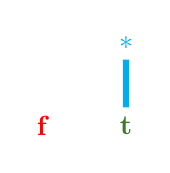
\begin{tikzpicture}[scale=0.35]
			\node (A) at (0,0) {\textcolor{red}{\textbf{f}}};
			\node (B) at (3,0) {\textcolor{OliveGreen}{\textbf{t}}};
			\node (C) at (3,3) {\textcolor{cyan}{$*$}};
			\draw[cyan, line width=.03in] (B) -- (C);
			\end{tikzpicture} \\
			& 	
\begin{tikzpicture}[scale=0.4]
				\node (A) at (0,0) {\textcolor{black}{$\bigcdot$}};
				\node (a) at (0.5,0) {\textcolor{orange}{$\bullet$}};
				\node (b') at (0.5,0.5) {\textcolor{yellow}{$\bullet$}};
				\node (B) at (0,3) {\textcolor{black}{$\bigcdot$}};
				\node (b) at (0.5,3) {\textcolor{yellow}{$\bullet$}};
				\draw[black, line width=.03in] (A) -- (B);
			\end{tikzpicture}
			\arrow["{a_j}", curve={height=-6pt}, from=2-1, to=1-2]
			\arrow[curve={height=-4pt}, from=2-1, to=3-2]
			\arrow[squiggly, two heads, from=2-3, to=3-2]
			\arrow["{\langle a_i,\;a_0a_j \rangle}"', dashed, from=2-1, to=2-3]
			\arrow[squiggly, two heads, from=2-3, to=1-3]
			\arrow["{a_0}", from=1-2, to=1-3]
			\arrow["{\textfrak{r}}", from=2-3, to=2-4]
			\arrow[curve={height=6pt}, from=2-1, to=1-2]
			\arrow["{a_i}"', curve={height=6pt}, from=2-1, to=3-2]
		\end{tikzcd}
		\caption{The images of $a_i,a_j$ with $i,j \in \{0,1\}$ are displayed with bullets of matching color.}
	\end{figure}
	We discover that:
	\begin{gather*}
		\models_{\mathbb{FF_2}} \forall_{x:1_\bot} r(x,a_0). \\
		\not\models_{\mathbb{FF_2}} \forall_{x:1_\bot} r(x,a_1).
	\end{gather*}
\end{ex}		 

\newpage
Moving on to existential quantification, we aim to realize in analogy to $\forall$, the formula $\exists_{x:1_\bot} r(x,a_1)$:

\begin{ex}
	If we unfold the definitions, in order for $\exists_{x:1_\bot} r(x,a_1)$ to be true at stage $\textbf{1}_\bot$ there must exist an epi $e: D \twoheadrightarrow \textbf{1}_\bot$ and an arrow $D \xrightarrow{a} \textbf{1}_\bot$ such that $D \VDashA r(a,  \;a_1e)$.
	\newline
	Let $D=\textbf{1}_\bot$,$e=a_1$ and $a=a_1$.
	\begin{figure}[h]
		\centering
		\begin{tikzcd}
			& {\textbf{1}_\bot} & {\textbf{1}_\bot} \\
			{D=\textbf{1}_\bot} && {\textbf{1}_\bot \times \textbf{1}_\bot} & \Omega \\
			& {\textbf{1}_\bot}
			\arrow["{e=a_1}", two heads, from=2-1, to=1-2]
			\arrow[squiggly, two heads, from=2-3, to=3-2]
			\arrow["{\langle a_1, a_1 a_1 \rangle}"', dashed, from=2-1, to=2-3]
			\arrow[squiggly, two heads, from=2-3, to=1-3]
			\arrow["{a_1}", from=1-2, to=1-3]
			\arrow["{\textfrak{r}}", from=2-3, to=2-4]
			\arrow["{a=a_1}"', from=2-1, to=3-2]
		\end{tikzcd}
	\end{figure}
		\begin{figure}[h]
		\centering
		\begin{tikzcd}
			& 
\begin{tikzpicture}[scale=0.4]
				\node (A) at (0,0) {\textcolor{black}{$\bigcdot$}};
				\node (a) at (0.5,0) {\textcolor{orange}{$\bullet$}};
				\node (B) at (0,3) {\textcolor{black}{$\bigcdot$}};
				\node (b) at (0.5,3) {\textcolor{yellow}{$\bullet$}};
				\draw[black, line width=.03in] (A) -- (B);
			\end{tikzpicture} & 
\begin{tikzpicture}[scale=0.4]
			\node (A) at (0,0) {\textcolor{black}{$\bigcdot$}};
			\node (a) at (0.5,0) {\textcolor{orange}{$\bullet$}};
			\node (B) at (0,3) {\textcolor{black}{$\bigcdot$}};
			\node (b) at (0.5,3) {\textcolor{yellow}{$\bullet$}};
			\draw[black, line width=.03in] (A) -- (B);
			\end{tikzpicture} \\
		
\begin{tikzpicture}[scale=0.4]
			\node (A) at (0,0) {\textcolor{OliveGreen}{$\bigcdot$}};
			\node (a) at (0.5,0) {\textcolor{orange}{$\bullet$}};
			\node (B) at (0,3) {\textcolor{OliveGreen}{$\bigcdot$}};
			\node (b) at (0.5,3) {\textcolor{yellow}{$\bullet$}};
			\draw[OliveGreen, line width=.03in] (A) -- (B);
		\end{tikzpicture} &&	
\begin{tikzpicture}[scale=0.35]
		\node (A) at (0,0) {\textcolor{OliveGreen}{$\bigcdot$}};
		\node (a) at (0.5,0) {\textcolor{orange}{$\bullet$}};
		\node (B) at (-3,3) {\textcolor{OliveGreen}{$\bigcdot$}};
		\node (b) at (0.5,3) {\textcolor{yellow}{$\bullet$}};
		\node (C) at (0,3) {\textcolor{OliveGreen}{$\bigcdot$}};
		\node (D) at (3,3) {\textcolor{cyan}{$\bigcdot$}};
		\draw[OliveGreen, line width=.03in] (A) -- (B);
		\draw[OliveGreen, line width=.03in] (A) -- (C);
		\draw[cyan, line width=.03in] (A) -- (D);
		\end{tikzpicture} & 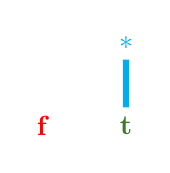
\begin{tikzpicture}[scale=0.35]
		\node (A) at (0,0) {\textcolor{red}{\textbf{f}}};
		\node (B) at (3,0) {\textcolor{OliveGreen}{\textbf{t}}};
		\node (C) at (3,3) {\textcolor{cyan}{$*$}};
		\draw[cyan, line width=.03in] (B) -- (C);
		\end{tikzpicture} \\
			& 
\begin{tikzpicture}[scale=0.4]
				\node (A) at (0,0) {\textcolor{black}{$\bigcdot$}};
				\node (a) at (0.5,0) {\textcolor{orange}{$\bullet$}};
				\node (B) at (0,3) {\textcolor{black}{$\bigcdot$}};
				\node (b) at (0.5,3) {\textcolor{yellow}{$\bullet$}};
				\draw[black, line width=.03in] (A) -- (B);
			\end{tikzpicture}
			\arrow["{e=a_1}", two heads, from=2-1, to=1-2]
			\arrow[squiggly, two heads, from=2-3, to=3-2]
			\arrow["{\langle a_1, a_1 a_1 \rangle}"', dashed, from=2-1, to=2-3]
			\arrow[squiggly, two heads, from=2-3, to=1-3]
			\arrow["{a_1}", from=1-2, to=1-3]
			\arrow["{\textfrak{r}}", from=2-3, to=2-4]
			\arrow["{a=a_1}"', from=2-1, to=3-2]
		\end{tikzcd}
	\caption{The usual coloring notation is applied.}	
	\end{figure}
	\newline
	This results in:
	\begin{gather*}
		\models_{\mathbb{FF_2}} \exists_{x:1_\bot} r(x,a_1). \\
		\models_{\mathbb{FF_2}} \exists_{x:1_\bot} r(x,a_0). \\
	\end{gather*}
\end{ex} 

We present a final example in which we introduce a new type $A' := \textbf{1}_\bot + \textbf{1}$ and a new relation $r'$ which \emph{extends} $r$ and is realized by $\textbf{1}_\bot \times \textbf{A}' \xrightarrow{\textfrak{r}'} \Omega$.
\begin{ex}
	We want to check the validity of $\exists_{x: 1_\bot} r(x,a'_2)$:
	\begin{figure}[h]
		\centering
		\begin{tikzcd}
			& 
\begin{tikzpicture}[scale=0.4]
				\node (A) at (0,0) {\textcolor{black}{$\bigcdot$}};
				\node (a) at (0.5,0) {\textcolor{orange}{$\bullet$}};
				\node (B) at (0,3) {\textcolor{black}{$\bigcdot$}};
				\node (b) at (0.5,3) {\textcolor{yellow}{$\bullet$}};
				\draw[black, line width=.03in] (A) -- (B);
			\end{tikzpicture} & 
\begin{tikzpicture}[scale=0.4]
				\node (A) at (0,0) {\textcolor{black}{$\bigcdot$}};
				\node (B) at (0,3) {\textcolor{black}{$\bigcdot$}};
				\node (C) at (2,0) {\textcolor{black}{$\bigcdot$}};
				\node (a) at (2.5,0) {\textcolor{orange}{$\bullet$}};
				\node (b) at (2.5,0.5) {\textcolor{yellow}{$\bullet$}};
				\draw[black, line width=.03in] (A) -- (B);
			\end{tikzpicture} \\
			
\begin{tikzpicture}[scale=0.4]
				\node (A) at (0,0) {\textcolor{red}{$\bigcdot$}};
				\node (a) at (0.5,0) {\textcolor{orange}{$\bullet$}};
				\node (B) at (0,3) {\textcolor{red}{$\bigcdot$}};
				\node (b) at (0.5,3) {\textcolor{yellow}{$\bullet$}};
				\draw[red, line width=.03in] (A) -- (B);
			\end{tikzpicture} &&	
\begin{tikzpicture}[scale=0.35]
				\node (A) at (0,0) {\textcolor{OliveGreen}{$\bigcdot$}};
				\node (B) at (-3,3) {\textcolor{OliveGreen}{$\bigcdot$}};
				\node (C) at (0,3) {\textcolor{OliveGreen}{$\bigcdot$}};
				\node (D) at (3,3) {\textcolor{cyan}{$\bigcdot$}};
				\node (E) at (5,0) {\textcolor{red}{$\bigcdot$}};
				\node (F) at (5,3) {\textcolor{red}{$\bigcdot$}};
					\node (a) at (5.5,0) {\textcolor{orange}{$\bullet$}};
					\node (b) at (5.5,0.5) {\textcolor{yellow}{$\bullet$}};
					\node (b') at (5.5,3) {\textcolor{yellow}{$\bullet$}};
				\draw[OliveGreen, line width=.03in] (A) -- (B);
				\draw[OliveGreen, line width=.03in] (A) -- (C);
				\draw[cyan, line width=.03in] (A) -- (D);
				\draw[red, line width=.03in] (E) -- (F);
			\end{tikzpicture} & 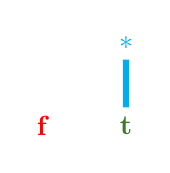
\begin{tikzpicture}[scale=0.35]
				\node (A) at (0,0) {\textcolor{red}{\textbf{f}}};
				\node (B) at (3,0) {\textcolor{OliveGreen}{\textbf{t}}};
				\node (C) at (3,3) {\textcolor{cyan}{$*$}};
				\draw[cyan, line width=.03in] (B) -- (C);
			\end{tikzpicture} \\
			& 
\begin{tikzpicture}[scale=0.4]
				\node (A) at (0,0) {\textcolor{black}{$\bigcdot$}};
				\node (a) at (0.5,0) {\textcolor{orange}{$\bullet$}};
				\node (B) at (0,3) {\textcolor{black}{$\bigcdot$}};
				\node (b) at (0.5,3) {\textcolor{yellow}{$\bullet$}};
				\draw[black, line width=.03in] (A) -- (B);
			\end{tikzpicture}
			\arrow["{e=a_1}", two heads, from=2-1, to=1-2]
			\arrow[squiggly, two heads, from=2-3, to=3-2]
			\arrow["{\langle a_1, a_1 a_1 \rangle}"', dashed, from=2-1, to=2-3]
			\arrow[squiggly, two heads, from=2-3, to=1-3]
			\arrow["{a'_2}", from=1-2, to=1-3]
			\arrow["{\textfrak{r}}", from=2-3, to=2-4]
			\arrow["{?a}"', from=2-1, to=3-2]
		\end{tikzcd}
		\caption{In this case $?a$ can be either $a_0$ or $a_1$.}	
	\end{figure}
	\newline
	This results in:
	\begin{equation*}
		\not\models_{\mathbb{FF_2}} \exists_{x:1_\bot} r'(x,a'_2).
	\end{equation*}
\end{ex}


\newpage
\subsection{\hl{Recovering First-Order $\mathcal{G}_3$}}		

Let's take a look back at what we found using BKJ Semantics.	
		Notice that:
		\begin{remark}
			In order to establish the validity of the universal quantified predicate $\forall_{x:1_\bot} p(x)$ we have to \emph{check} a \emph{finite} number of generalized elements $a_i$.
			In fact, this was equivalent to checking if $\textbf{1}_\bot \VDashA p(a_0)$ and $\textbf{1}_\bot \VDashA p(a_1)$  i.e., if $\textbf{1}_\bot \VDashA p(a_0) \land p(a_1) $ which is equivalent to establishing if $\models_{\mathbb{FF_2}} p(a_0) \land p(a_1) $.
		\end{remark}
		Also:
		\begin{remark}
			 The same phenomenon occurs in order to establish the validity of a universal quantified relation $\forall_{x:1_\bot} r(x,a_0)$. We also have to \emph{check} a \emph{finite} number of generalized elements $a_i,a_j$.
			In fact, this was equivalent to checking if $\textbf{1}_\bot \VDashA r(a_1,a_0)$ and $\textbf{1}_\bot \VDashA r(a_0,a_0)$  i.e., if 
			$\textbf{1}_\bot \VDashA r(a_0,a_0) \land r(a_1,a_0)$ which in turn is equivalent to establishing if $\models_{\mathbb{FF_2}} r(a_0,a_0) \land r(a_1,a_0) $.
		\end{remark} 
		 
		 This suggests that:
		 \begin{lem}
		 	The semantics of a universally quantified formula in $\mathbb{FF_2}$ correspond to  finitary\footnote{\emph{bushes}, recall, are \emph{finite} forests.} conjunction of instanced formulae.
		 	\footnote{the instances to consider are those of $\phi(a_i,..)$ where $x_i : A_i$ is the variable being quantified over and $a_i$ is a generalized element of $A_i$.} 
		 \end{lem}
		 
In a similar manner:

\begin{remark}
	In order to establish the validity of the existential quantified predicate $\exists_{x:1_\bot} p(x)$ we have to \emph{check} a \emph{finite} number of generalized elements $a_i$. 
	In fact, this was equivalent to checking if either $\textbf{1}_\bot \VDashA p(a_0)$ or $\textbf{1}_\bot \VDashA p(a_1)$  i.e., if $\textbf{1}_\bot \VDashA p(a_0) \lor p(a_1) $ which is equivalent to establishing if $\models_{\mathbb{FF_2}} p(a_0) \lor p(a_1) $.
\end{remark}

Now, a categorical consideration:

\begin{lem}
	$\textbf{1}_\bot$ is \emph{indecomposable}.
\end{lem} 
	This becomes quite apparent as the epis in $\mathbb{FF}_*$ are the surjective arrows. Assuming $[k,l] : D + E \twoheadrightarrow \textbf{1}_\bot$ is an epi, if neither $D \xrightarrow{k} \textbf{1}_\bot$ nor $E \xrightarrow{l} \textbf{1}_\bot$ are epis then they must both be constant maps into the root of $\textbf{1}_\bot$ and so $[k,l]$ must be a constant map into the root of $\textbf{1}_\bot$ which brings us to a contradiction.

\begin{remark}
	In order to establish the validity of the existential quantified formula $\exists_{x:1_\bot} r(x,a_0)$ we have to \emph{check} a \emph{finite} number of generalized elements $a_i,a_j$. \newline
	In fact, this was equivalent to checking if either $\textbf{1}_\bot \VDashA r(a_1,a_0)$ or $\textbf{1}_\bot \VDashA r(a_0,a_0)$  i.e., if $\textbf{1}_\bot \VDashA r(a_0,a_0) \lor r(a_1,a_0) $ which in turn is equivalent to establishing if $\models_{\mathbb{FF_2}} r(a_0,a_0) \lor r(a_1,a_0) $.
\end{remark} 

This suggests, analogously to the previous case:

\begin{lem}
	The semantics of an existentially quantified formula in $\mathbb{FF_2}$ corresponds to a generalized finitary disjunction of instanced formulae.
\end{lem}

Finally, let us observe that:

\begin{remark}
	$\mathbb{FF_2}$-validity of instanced atomic formulae like $\phi(a_1,..,a_n)$ is always reduced to $\mathbb{FF_2}$-validity at the stage $\textbf{1}_\bot$ which in turn corresponds to checking if the fiber of $t$ by $\top !_{1_\bot}$ coincides with the maximal sub-forest of $\textbf{1}_\bot$ i.e., $(\top !_{1_\bot})^{-1}[t] = \{\textbf{1}_\bot\}$.
\end{remark}
\newpage
Recall now that $Sub(\textbf{1}_\bot) \cong C_3$ and semantically characterizes $\mathcal{G}_3$.
 \begin{figure}[h]
	\centering
	\begin{tikzpicture}[thick,scale=0.6, every node/.style={scale=0.8}]
		\node (A) at (0,0) {\textcolor{red}{$\emptyset$}};
		\node (B) at (0,2) {\textcolor{cyan}{$\{ \bot \}$}};
		\node (C) at (0,4) {\textcolor{OliveGreen}{$\{ \textbf{1}_\bot \}$}};
		\draw[line width=.01in] (A) -- (B);
		\draw[line width=.01in] (B) -- (C);
		\node (D) at (4,0) {\textcolor{black}{$\bot$}};
		\node (E) at (4,2) {\textcolor{black}{$\bigcdot$}};
		\draw[line width=.01in] (D) -- (E);
	\end{tikzpicture}
	\caption{ $Sub(\textbf{1}_\bot)$ (left) and $\textbf{1}_\bot$ (right).}
\end{figure}

\begin{remark}
We can define an assignment $\mathcal{A}$ from instanced atomic formulae $\phi$ to the Gödel set $\textfrak{T}= \{0, \frac{1}{2}, 1\}$ whereby if we consider the sub-forest of $\textbf{1}_\bot$ determined by  $(\top !_{1_\bot})^{-1}[t]$:
			\begin{equation*}
				\mathcal{A}(\phi) := \begin{cases}
					1 &	\text{if } (\top !_{1_\bot})^{-1}[t] = \{\textbf{1}_\bot\} \\
					\frac{1}{2} & \text{if } (\top !_{1_\bot})^{-1}[t] = \{\bot\}  \\
					0 & \text{if } (\top !_{1_\bot})^{-1}[t] = \emptyset 
				\end{cases}     .  
			\end{equation*}
\end{remark}

Recall also that the semantics of first order $\mathcal{G}_3$ in \ref{fosemantics} whereby $\forall$ and $\exists$ where essentially interpreted as generalized $\land$ and $\lor$, i.e., the interpretation of $\forall x. A(x)$ and $\exists x.A(x)$ was respectively the $min$ and $max$ of the interpretations of the instances $A(u)$ where $u$ ranged over some domain or universe $\textfrak{U}$.
\newline\newline
This suggests, summing up all these results, the following:

\begin{thm}[first-order logic of $\mathbb{FF_2}$]
${}$ \newline
The first-order logic of the topos of $\mathbb{FF_2}$/\emph{bushes} corresponds to first-order three-valued Gödel-Dummett Logic on \emph{finite} domains.  
\end{thm}		 

In other words:	 
\begin{remark}
	The topos of \emph{bushes} provides first order finite models for three-valued Gödel-Dummett Logic.
\end{remark}		 
		 
		 
	\newpage
${}$ \newpage		 